% $Header: /cvsroot/latex-beamer/latex-beamer/solutions/generic-talks/generic-ornate-15min-45min.en.tex,v 1.5 2007/01/28 20:48:23 tantau Exp $

\documentclass{beamer}

\usepackage{caption}
\captionsetup{labelformat=empty,labelsep=none,font=scriptsize}
\setlength{\abovecaptionskip}{0pt}

\usepackage{color}
%% These definitions are based on darkred at
%% http://www.december.com/html/spec/colorcmyk.html
\definecolor{darkred}{cmyk}{0, 1, 1, 0.45}

% This file is a solution template for:

% - Giving a talk on some subject.
% - The talk is between 15min and 45min long.
% - Style is ornate.



% Copyright 2004 by Till Tantau <tantau@users.sourceforge.net>.
%
% In principle, this file can be redistributed and/or modified under
% the terms of the GNU Public License, version 2.
%
% However, this file is supposed to be a template to be modified
% for your own needs. For this reason, if you use this file as a
% template and not specifically distribute it as part of a another
% package/program, I grant the extra permission to freely copy and
% modify this file as you see fit and even to delete this copyright
% notice. 


\mode<presentation>
{
  \usetheme{Warsaw}
  % or ...

  \setbeamercovered{transparent}
  % or whatever (possibly just delete it)
}


\usepackage[english]{babel}
% or whatever

\usepackage[latin1]{inputenc}
% or whatever

\usepackage{times}
\usepackage[T1]{fontenc}
% Or whatever. Note that the encoding and the font should match. If T1
% does not look nice, try deleting the line with the fontenc.


%% \title[Short Paper Title] % (optional, use only with long paper titles)
%% {Presentation Title}
%% \title[]{Initial findings}
%\subtitle {Eastern CASTNET sites, May-Sep.~2001} % (optional)

%% \author[Author, Another] % (optional, use only with lots of authors)
%% {F.~Author\inst{1} \and S.~Another\inst{2}}
%% % - Use the \inst{?} command only if the authors have different
%% %   affiliation.
%% \author[Swall et al.]{Jenise Swall\inst{1}, Ana Rappold\inst{2}, and Lucas Neas\inst{2}
% - Use the \inst{?} command only if the authors have different
%   affiliation.

%% \institute[Universities of Somewhere and Elsewhere] % (optional, but mostly needed)
%% {
%%   \inst{1}%
%%   Department of Computer Science\\
%%   University of Somewhere
%%   \and
%%   \inst{2}%
%%   Department of Theoretical Philosophy\\
%%   University of Elsewhere}
%% % - Use the \inst command only if there are several affiliations.
%% % - Keep it simple, no one is interested in your street address.
 %% \institute[VCU]
 %% {
 %%   \inst{1}%
 %%   Dept.\ of Statistical Sciences and Operations Research\\
 %%   Virginia Commonwealth University
 %%   \and
 %%   \inst{2}%
 %%   National Health and Environmental Effects Research Laboratory\\
 %%   U.S.~Environmental Protection Agency
 %% }

%% \date[Short Occasion] % (optional)
%% {Date / Occasion}
\date{Mar.\ 2020}

%% \subject{Talks}
% This is only inserted into the PDF information catalog. Can be left
% out. 



% If you have a file called "university-logo-filename.xxx", where xxx
% is a graphic format that can be processed by latex or pdflatex,
% resp., then you can add a logo as follows:

% \pgfdeclareimage[height=0.5cm]{university-logo}{university-logo-filename}
% \logo{\pgfuseimage{university-logo}}



% Delete this, if you do not want the table of contents to pop up at
% the beginning of each subsection:
\AtBeginSection[]
{
  \begin{frame}<beamer>{Outline}
    \tableofcontents[currentsection,currentsubsection]
  \end{frame}
}


% If you wish to uncover everything in a step-wise fashion, uncomment
% the following command: 

%\beamerdefaultoverlayspecification{<+->}

\useoutertheme{infolines}

\begin{document}

%% \begin{frame}
%%   \titlepage
%% \end{frame}

\begin{frame}{Outline}
  \tableofcontents
  % You might wish to add the option [pausesections]
\end{frame}


% Since this a solution template for a generic talk, very little can
% be said about how it should be structured. However, the talk length
% of between 15min and 45min and the theme suggest that you stick to
% the following rules:  

% - Exactly two or three sections (other than the summary).
% - At *most* three subsections per section.
% - Talk about 30s to 2min per frame. So there should be between about
%   15 and 30 frames, all told.


%% %%%%%%%%%%%%%%%%%%%%%%%%%%%%%%%%%%%%%%%%%%%%%%%%%%%%%%%%%%



%% %%%%%%%%%%%%%%%%%%%%%%%%%%%%%
%% Introductory material
%% \section[Background]{Background ideas and info}
\section{Organizing the data}


\begin{frame}{Which taxa were included?}

  {\footnotesize
    \begin{itemize}
    \item When working with the bacteria counts, I only considered
      taxa which could be classified to the family level.
    \item In the case of the eukaryotes, many taxa could not be
      classified at the family level, so all taxa (e.g., ``\_fa'',
      ``\_unclassified'') were considered at the outset.
    \item For each sample, we calculated the total counts of all taxa
      (5287 for all).  Then, we calculated the fraction of counts
      associated with each taxon.  (Fractions, not counts, were used
      in the model.)
    \item To be included in the random forest model, I required that
      a taxon must make up more than 1\% of the total counts for at least
      2 samples.
     \item This process was done separately for ribs and scapulae, so
       the taxa used in their random forest models differed.
    \end{itemize}
  }
  
\end{frame}



\begin{frame}{Taxa for the rib model}

  {\footnotesize
    
  \noindent  Fourteen taxa were used in the random forest model for ribs.
  
  \vspace{0.1in}

  \noindent These 14 taxa were:
  
  \vspace{0.05in}

  \begin{tabular}{ll}
    Armophorea\_unclassified & Armophorida\\
    Arthropoda\_unclassified & Bacillariophyceae\\
    Chromadorea\_unclassified & Diatomea\_unclassified\\
    Eukaryota\_unclassified &  Haplotaxida\_fa\\
    Hypotrichia & Intramacronucleata\_unclassified\\
    Mediophyceae & Melosirids\\
    Oligohymenophorea & Peronosporomycetes\_fa          
  \end{tabular}

  \vspace{0.2in}
  \noindent There are only 59 observations available for the rib data.
  \begin{itemize}
    \item There are no rib samples for collections 7 and 17 (ADD 1827 and 4473).
    \item There is only 1 rib sample for collections 1, 2, and 6 (ADD 268, 516,
    and 1513).
    \item There are 2 rib samples for collections 5 and 9 (ADD 1278 and 2395).
    \item The last 6 collections (after ADD 3181) have 4-5 rib samples at each
    collection.
  \end{itemize}
  }

\end{frame}



\begin{frame}{Taxa for the scapula model}

  {\scriptsize
    
  \noindent Twenty-one taxa were used in the random forest model for
  scapulae.
  
  \vspace{0.1in}

  \noindent These 21 taxa were:
  
  \vspace{0.05in}

  \begin{tabular}{ll}
    Armophorea\_unclassified         & Armophorida\\                   
    Arthropoda\_unclassified         & Bacillariophyceae\\              
    Chromadorea\_unclassified        & Clitellata\_unclassified\\        
    Continenticola\_fa               & Diatomea\_unclassified\\         
    Eukaryota\_unclassified          & Haplotaxida\_fa\\         
    Haptoria                         & Heterobranchia\_fa\\              
    Hypotrichia                      & Intramacronucleata\_unclassified\\
    Mediophyceae                     & Melosirids\\                     
    Metakinetoplastina\_unclassified & Oligohymenophorea\\              
    Peronosporomycetes\_fa           & Podocopida\_fa\\             
  \end{tabular}

  \vspace{0.2in}
  \noindent There are 87 observations available for the scapula data.
  \begin{itemize}
    \item There is only 1 scapula sample for collection 17 (ADD 4473).
    \item Other than collection 17, all other collection days included 4 or 5
    scapula samples.
  \end{itemize}
  }

\end{frame}
%% %%%%%%%%%%%%%%%%%%%%%%%%%%%%%



%% %%%%%%%%%%%%%%%%%%%%%%%%%%%%%
\section[Ribs]{Analysis using Rice Rivers ribs}


\begin{frame}{Implementing the random forest model for ribs}

  \begin{itemize}
  \item The model utilized 14 family-level taxa.
  \item Cross-validation was used to determine that the best number of
    taxa to consider at each "branching" of the trees.  This turned out to be
    14, which means all taxa were considered at each "branching".
  \end{itemize}

  \vspace{0.1in}

  \begin{itemize}
  \item Because of the ``random'' component inherent in random forest
    models, each fitted model is a little different.
  \item To get an idea of this variability, I fit the random forest
    model over and over, calculating the root mean squared error
    (RMSE) and percentage of variation explained for each.
  \end{itemize}

  \vspace{0.1in}
  
  \noindent RMSE: 545.9 $\pm$ 6.4 \hspace{0.2in}  Explained variation: 84.3\% $\pm$ \%0.4

\end{frame}



\begin{frame}{Influential taxa}

  \begin{center}
    \begin{figure}
      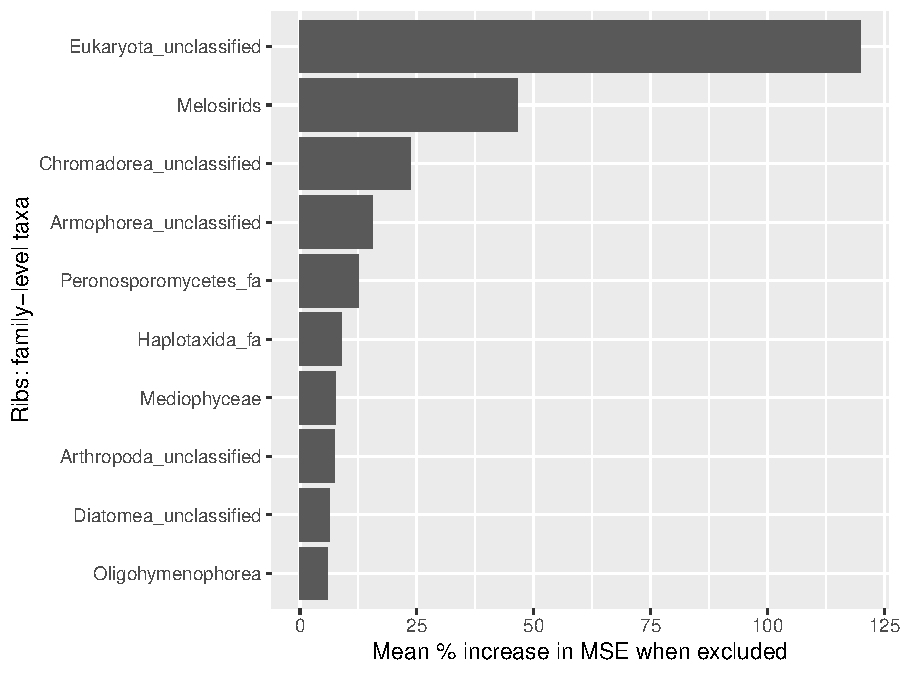
\includegraphics[width=2.25in]{w_ribs/families_rib_PercIncMSE_barchart}
    \end{figure}
  \end{center}
  
  {\scriptsize
    \begin{itemize}
    \item The measure of importance is the mean percentage increase in
      the mean-square error of model predictions when the variable is
      left out of the model.
    \item I've shown the top 10 because they fit easily.
    \item The most influential taxa is Eukaryota\_unclassified, which I find
    concerning.  This is saying that the percentage of taxa that are
    unclassifiable is the most predictive taxon.
    \item The next most influential taxon is Melosirids, but it's much less
    influential than Eukaryota\_unclassified.
    \end{itemize}
  }

\end{frame}



\begin{frame}{Scatterplots for influential taxa}

  \begin{center}
    \begin{figure}
      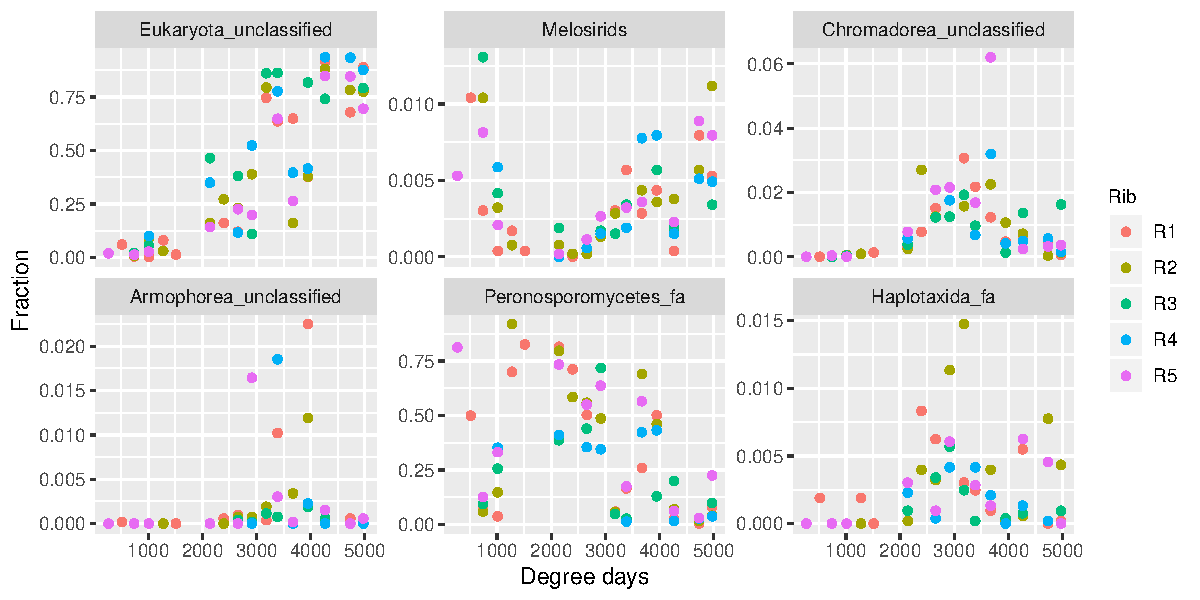
\includegraphics[width=4.5in]{w_ribs/infl_rib_family_scatter}
    \end{figure}
  \end{center}
  \vspace{-0.2in}
  {\scriptsize
  \begin{itemize}
  \item I've only shown the top 6 because more than that is hard to fit.
  \item Note that the y-axes have differing scales.
  \item We can see that Eukaryota\_unclassified steadily increases over the
  study period, which is why it's so influential.
  \item Fractions of Armophorea\_unclassified and Haplotaxida\_unclassified are
  very low throughout.
  \end{itemize}
  }

\end{frame}



\begin{frame}{Getting a sense of "real-life" model fit}

  \noindent In real life, we would be estimating ADD without
  \begin{itemize}
    \item having seen that rib/scapula before, and
    \item maybe not having observed any rib/scapula at that level of ADD before
  \end{itemize} 

  \vspace{0.1in}

  \noindent To try to get a sense of how the model would work in such cases, I
  \begin{itemize}
    \item fitted the model over and over, each time without one particular
    combination of rib/scapula number and ADD.
    \item This means the model had no info about the left-out rib/scapula and no
    info about bacteria counts at that ADD.
    \item Then, I used the model to estimate the ADD for the left-out
    rib/scapula for the left-out ADD.
  \end{itemize}
  
\end{frame}



\begin{frame}{Residual plot to get sense of "real-life" model fit}

  \begin{center}
  \begin{figure}
    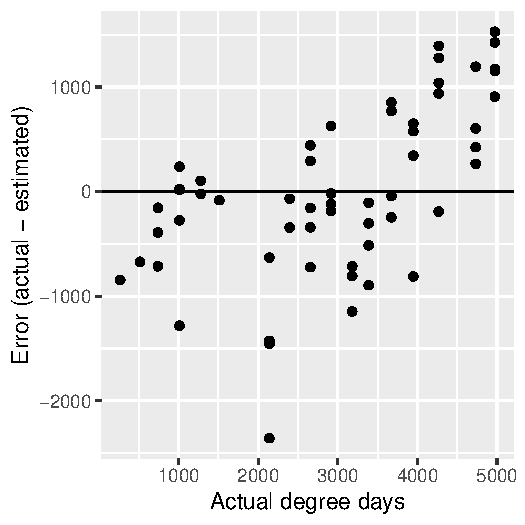
\includegraphics[width=1.5in]{w_ribs/leave_out_one_rib_and_one_day_residuals}
  \end{figure}
  \end{center}  

  \vspace{0.1in}

  {\scriptsize
 
    \begin{itemize}
    \item This RMSE is in the range of 817-819, which is higher than
      the RMSE for the model fitted on the full dataset (as you'd expect).  We
      have less data available for each run, and we're predicting for an ADD
      value which we have no information about.
    \item We expect that errors tend to be larger at the extremes, but here we
    also have large errors for ADD 2141.  This is probably because we have
    limited samples for the neighboring collections.  (We have no rib data for
    ADD 1827, 1 sample for 1513, and 2 samples for 2395.)
    \end{itemize}
  }

\end{frame}
%% %%%%%%%%%%%%%%%%%%%%%%%%%%%%%




%% %%%%%%%%%%%%%%%%%%%%%%%%%%%%%
\section[Scapulae]{Analysis using Rice Rivers scapulae}

\begin{frame}{Implementing the random forest model for scapulae}

  \begin{itemize}
  \item The model utilized 21 family-level taxa.
  \item Cross-validation was used to determine that the best number of
    taxa to consider at each "branching" of the trees (about 9).
  \end{itemize}

  \vspace{0.1in}

  \begin{itemize}
  \item Because of the ``random'' component inherent in random forest
    models, each fitted model is a little different.
  \item To get an idea of this variability, I fit the random forest
    model over and over, calculating the root mean squared error
    (RMSE) and percentage of variation explained for each.
  \end{itemize}

  \vspace{0.1in}
  
  \noindent RMSE: 526.0  $\pm$ 5.3 \hspace{0.2in}  Explained variation: 86.0\% $\pm$ \%0.3

\end{frame}



\begin{frame}{Influential taxa}

  \begin{center}
    \begin{figure}
      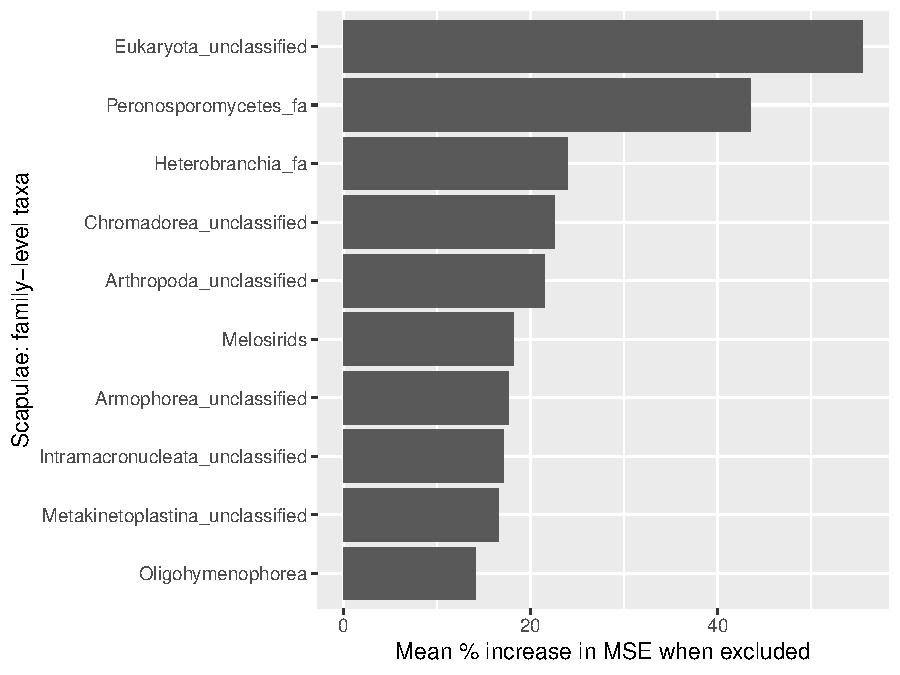
\includegraphics[width=2.25in]{w_scapulae/families_scapula_PercIncMSE_barchart}
    \end{figure}
  \end{center}

  \vspace{0.05in}
  
  {\scriptsize
    \begin{itemize}
    \item Again, I've just shown the top 10.
    \item As with the ribs, Eukaryota\_unclassified is the most
      influential taxon.
    \item The second most influential taxon is Peronosporomycetes\_fa,
      which is different from that for the ribs.
    \item There is a large gap between Peronosporomycetes\_fa and the
      rest of the taxa.
  \end{itemize}
  }

\end{frame}



\begin{frame}{Scatterplots for influential taxa}

  \begin{center}
    \begin{figure}
      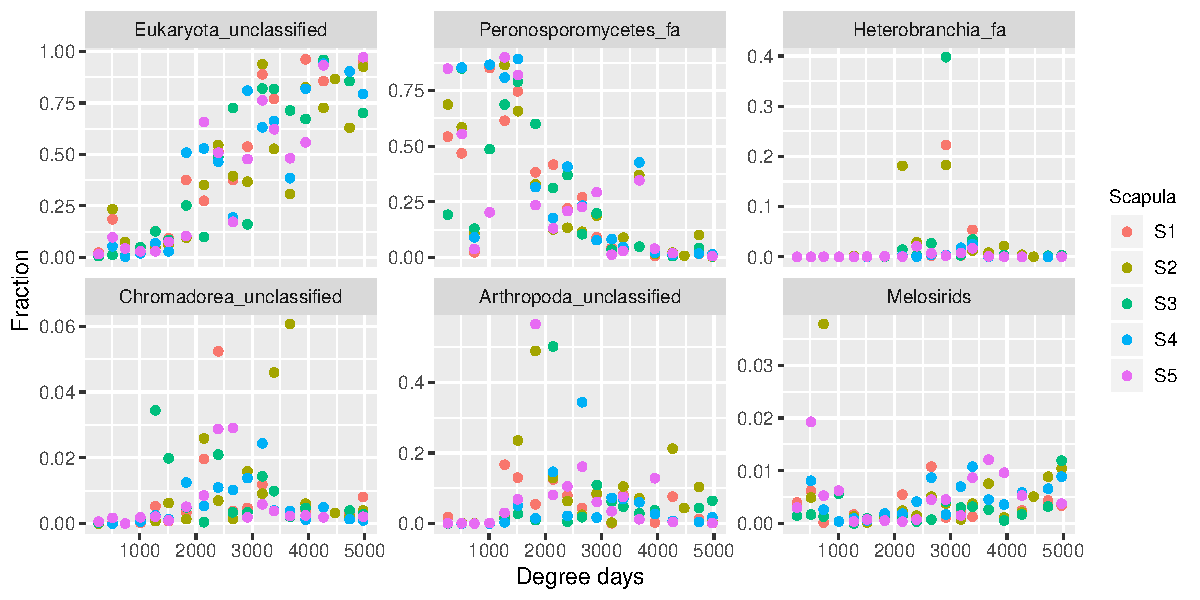
\includegraphics[width=4.75in]{w_scapulae/infl_scapula_family_scatter}
    \end{figure}
  \end{center}
  \vspace{-0.25in}
  {\scriptsize
  \begin{itemize}
  \item Again, I've only shown top 6.
  \item Note that the y-axes have differing scales.
  \item As with the ribs, we see that Eukaryota\_unclassified steadily increases
  over the study period, which is why it's so influential.
  \item Fractions of Melosirids are quite low, and this taxon does not have as
  much of an influential role as it does for the ribs.
  \end{itemize}
  }

\end{frame}



\begin{frame}{Residual plot to get sense of "real-life" model fit}

  \begin{center}
    \begin{figure}
      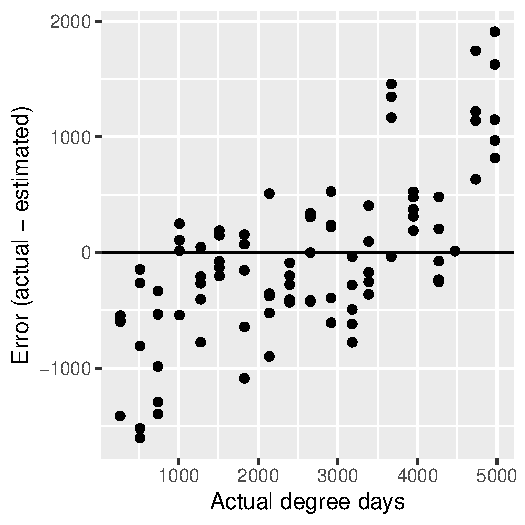
\includegraphics[width=1.5in]{w_scapulae/leave_out_one_scapula_and_one_day_residuals}
    \end{figure}
  \end{center}
  
  \vspace{0.1in}

  {\scriptsize
    \begin{itemize}
    \item The RMSE is in the range of 705-710.  As expected, this is
      higher than the RMSE for the full dataset.
    \item In general, this plot looks better than the corresponding one for the
    rib data.
    \item We do see some large residuals at ADD 3673.  This may be due to the
    fact that scapulae 2, 4, and 5 have somewhat low fractions of
    Eukaryota\_unclassified and quite high fractions of Peronosporomycetes\_fa
    on ADD 3673. 
    \end{itemize}
  }

\end{frame}
%% %%%%%%%%%%%%%%%%%%%%%%%%%%%%%


\end{document}
